%
% Modelo de relatório/trabalho
%
\documentclass[a4paper, 12pt]{article}

\usepackage[portuguese]{babel}
\usepackage[utf8]{inputenc}
\usepackage[T1]{fontenc}
\usepackage{array}
\usepackage{fixltx2e}
\usepackage{amsmath}
\usepackage{amssymb}
\usepackage{graphicx}
\usepackage{caption}
\usepackage{subcaption}
\usepackage{float}
\usepackage{a4wide}
\usepackage{courier}
\usepackage{multicol}
\usepackage[table]{xcolor}
\usepackage[htt]{hyphenat}
\usepackage{makeidx}
\usepackage{hyperref}
\usepackage{setspace}
\usepackage{indentfirst}
\usepackage[nottoc]{tocbibind}
\usepackage{listings}
\usepackage[bottom]{footmisc}
\usepackage[a4paper,top=2.0cm,bottom=2.0cm,left=1.83cm,right=2.0cm]{geometry}
\usepackage[square, sort, comma, numbers]{natbib}

\onehalfspacing
\graphicspath{{../diagrams/}}
\makeindex

\lstset{
    basicstyle=\footnotesize,
    morekeywords={either,or,transform,rule,to,from,through,function},
    frame=L,
}

\setcounter{secnumdepth}{2}
\setcounter{tocdepth}{2}

\begin{document}

\hypersetup{backref,pdfpagemode=FullScreen,colorlinks=true}

\title{EP1 --- MAC5742}
\author{Thilo Koch e Pedro Bruel}
\date{}
\maketitle

\section{Introdução} \label{sec:intro}

Este relatório descreve as atividades realizadas
para o EP1 da disciplina de Computação Paralela e
Distribuída (\textit{MAC5742}). A Seção \ref{sec:ex1}
descreve e corrige um exemplo encontrado num tutorial do padrão
OpenMP, e a Seção \ref{sec:ex2} descreve as modificações,
experimentos e interpretações feitos no código fornecido no enunciado.

Os diretórios \texttt{src}, \texttt{failing-example} e \texttt{doc}
contêm \textit{Makefiles} para geração dos executáveis e da documentação,
portanto basta executar o comando \texttt{make} para gerá-los.

\section{Exercício 1} \label{sec:ex1}

Neste exercício, procuramos um exemplo que contivesse falhas em um
tutorial, e tentamos corrigi-lo. O código do exemplo está na Seção
\ref{sec:example}, e nossa correção na Seção \ref{sec:fixed}.

Seguindo manual \textit{Guide into OpenMP: Easy multithreading
programming for C++}, na seção sobre OpenMP e \textit{fork()}
\footnotemark[1],
encontramos um exemplo que usa uma chamada a \textit{fork()} para criar um
subprocesso que utiliza cláusulas OpenMP.

O exemplo tem a intenção de demonstrar o uso \textit{incorreto} do OpenMP
com \textit{fork()}, mas não apresenta uma solução.
Nossa correção faz com que o programa execute da forma esperada (correta).

\subsection{Usando OpenMP e \textit{fork()}}

O problema deste exemplo é o uso de \textit{pragmas} OpenMP tanto
no processo pai como no processo filho. Segundo as discussões
encontradas em dois \textit{bugreports} do GCC
\footnotemark[2]\footnotemark[3],
o exemplo falha pois as \textit{thread pools} criadas pela \textbf{libgomp}
(\textit{GNU Offloading and Multi Processing Runtime Library})
\footnotemark[4] em cada
seção paralela (\textit{\#pragma omp parallel}) são passadas aos processos
filhos criados pela chamada a \textit{fork()}. No entanto, \textit{fork()}
não duplica as \textit{threads} e o processo filho não termina a execução,
entrando em \textit{deadlock} enquanto espera por \textit{threads} que não
existem em seu contexto.

As soluções apresentadas nas discussões nos \textit{bugreports} consistem
em modificar o código da \textbf{libgomp} para que ela destrua as
\textit{thread pools} antes da chamada a \textit{fork()}, chamando
\textit{pthread\_atfork()}, por exemplo. Porém, essas soluções não são
adequadas aos padrões \textbf{POSIX}, que exigem a manutenção dos valores
privados de \textit{threads} em chamadas a \textit{fork()}. Essas soluções
tornariam impossível reutilizar as \textit{threads} de uma \textit{thread pool}
criada antes de uma chamada a \textit{fork()}, por exemplo.

A solução correta para o uso de cláusulas OpenMP e chamadas a \textit{fork()}
é simplesmente não utilizar \textit{pragmas} no processo pai antes de
chamadas a \textit{fork}. Basta reorganizar o código para que os processos
filhos criem suas próprias \textit{thread pools} e não entrem em
\textit{deadlock}.
\footnotetext[1]{http://bisqwit.iki.fi/story/howto/openmp/\#OpenmpAndFork}
\footnotetext[2]{https://gcc.gnu.org/bugzilla/show\_bug.cgi?id=52303}
\footnotetext[3]{https://gcc.gnu.org/bugzilla/show\_bug.cgi?id=58378}
\footnotetext[4]{https://gcc.gnu.org/onlinedocs/libgomp/index.html}

\subsection{Código do Exemplo}\label{sec:example}
\begin{figure}[H]
    \centering
    \lstinputlisting[language=C, firstline=5, lastline=32]{../failing-example/fork_hangs.c}
    \caption{\texttt{failing-example/fork\_hangs.c}}
    \label{fig:fork_hangs}
\end{figure}

\subsection{Código Corrigido}\label{sec:fixed}
\begin{figure}[H]
    \centering
    \lstinputlisting[language=C, firstline=5, lastline=32]{../failing-example/fork.c}
    \caption{\texttt{failing-example/fork.c}}
    \label{fig:fork}
\end{figure}

\section{Exercício 2} \label{sec:ex2}

Neste exercício, fizemos modificações no arquivo \texttt{mult.c}, fornecido
no enunciado do EP1. O arquivo realiza uma multiplicação de matrizes,
e contém três laços aninhados.

Fizemos modificações para usar cláusulas OpenMP em cada um dos três laços.
Excertos do código implementado estão na Seção \ref{sec:code}. Depois,
testamos essas modificações em quatro arquiteturas diferentes, descritas
na Seção \ref{sec:arch}. Os resultados e sua discussão são apresentados,
respectivamente, nas Seções \ref{sec:res} e \ref{sec:dis}.

Os \textit{scripts} \texttt{measure\_par.py} e \texttt{measure\_seq.py}
realizam as medições dos arquivos com as modificações. O \textit{script}
\texttt{measure\_all.sh} realiza todas as medições utilizadas neste trabalho,
e o \textit{script} \texttt{produce\_diagrams.sh} gera os gráficos
apresentados.

\subsection{Arquiteturas e Configurações Utilizadas} \label{sec:arch}

Esta seção descreve as arquiteturas e configurações utilizadas nos experimentos.
Os diretórios \texttt{results/[nome\_da\_arquitetura]/} contêm arquivos
\texttt{[nome\_da\_arquitetura].txt}, que apresentam informações mais
detalhadas sobre cada uma.

\begin{itemize}
\item \textbf{HAL8k}: 
Processador com 6 \textit{cores} e HT: Debian Linux 3.2 x86\_64, AMD 
FX(tm)-6100 Six-Core Processor, gcc 4.7.2.
\item \textbf{hpops}: 
Processador com 2 \textit{cores} e HT: Debian Linux 3.2 x86\_64, 
Intel(R) Core(TM)2 Duo CPU E7500, gcc 4.7.2.
\item \textbf{hpops2}: 
Mesmo processador que \textbf{hpops}: Fedora 
Linux 3.19 x86\_64, gcc 4.9.3.
\item \textbf{hpops2\_50}: 
Mesmo \textit{setup} que \textbf{hpops2}: com 50 iterações (amostras) por 
tamanho de matriz.
\item \textbf{hpops2\_O3}: 
Mesmo \textit{setup} que \textbf{hpops2}: Compilado 
com gcc e a \textit{flag} \texttt{-O3}.
\item \textbf{mops}: 
Processador com 2 \textit{cores} e HT: Fedora Linux 3.18 x86\_64, 
Intel Core i5-2435M CPU, gcc 4.8.3.
\item \textbf{virtbox}: 
Máquina Virtual (VirtualBox) em \textbf{mops}:
Fedora Linux 3.18 x86\_64, Intel(R) Core(TM) i5-2435M CPU, gcc 4.8.3
\end{itemize}


\subsection{Paralelizações com OpenMP} \label{sec:code}

Esta seção apresenta as modificações que fizemos no arquivo
\texttt{mult.c}, paralelizando a multiplicação de matrizes
em cada um dos três níveis de laço aninhado.

Nos laços mais externos, utilizamos o \textit{pragma omp parallel for},
especificando que cada \textit{thread} terá seus índices de
acesso privados, através do parâmetro \textit{private}.

No laço mais interno, utilizamos uma variável temporária para que pudéssemos
utilizar o parâmetro \textit{reduction}, que não pode ser usado nos elementos
da matriz \textit{c}. A seguir está o código da nossa implementação com a
variável temporária.

\subsubsection{Paralelização do Laço mais Interno}

\begin{figure}[H]
    \centering
    \lstinputlisting[language=C, firstline=60, lastline=69]{../src/mult_par_v1.c}
    \caption{\texttt{src/mult\_par\_v1.c}}
    \label{fig:par_v1}
\end{figure}

\subsection{Resultados} \label{sec:res}

Esta Seção apresenta os resultados obtidos nas arquiteturas \textbf{hpops}
(e variações), \textbf{mops} e \textbf{HAL8k} --- ver Seção \ref{sec:arch}.
Em cada Subseção, são apresentados os respectivos gráficos e discussão dos
resultados. Os valores dos pontos em cada gráfico são a média ao longo de
10 medições, como especificado no enunciado.

Alguns resultados foram omitidos por conta da falta de espaço na
documentação, mas estão armazenados em arquivos
\texttt{[nome\_da\_arquitetura].result}, nos diretórios
\texttt{result/[nome\_da\_arquitetura]/}. As arquiteturas

\subsubsection{Uma \textit{thread} OpenMP vs. Algoritmo Sequencial}

Neste experimento é possível ver o \textit{overhead} causado pelo uso das
diretivas de compilação. A versão sequencial de \texttt{mult.c} foi mais rápida
do que as versões com uma \textit{thread}, em todos os tamanhos de matriz, nas
arquiteturas \textbf{hpops2} (Figura \ref{fig:hpops2_cmp_single}) e
\textbf{hpops2\_O3}(Figura \ref{fig:hpops2_O3_cmp_single}). Na arquitetura
\textbf{HAL8k} (Figura \ref{fig:8k_cmp_single}), por outro lado, podemos
observar que a versão com uma única \textit{thread} OpenMP ganha da
versão sequencial, para tamanhos de matriz grandes o suficiente. Nossa
interpretação é que essa diferença não é significativa, pois é devida a
variações nas medições.

Na arquitetura \textbf{hpops2\_O3}, vemos que a otimização do GCC \texttt{-O3}
produziu \textit{speedups} para todas as versões, inclusive a sequencial.
Essa otimização beneficiou mais as versões sequencial, de paralelização do
laço do meio, e de paralelização do laço mais externo, em matrizes de tamanho
pequeno.

\begin{figure}[H]
    \centering
    \begin{subfigure}[H]{0.5\textwidth}
        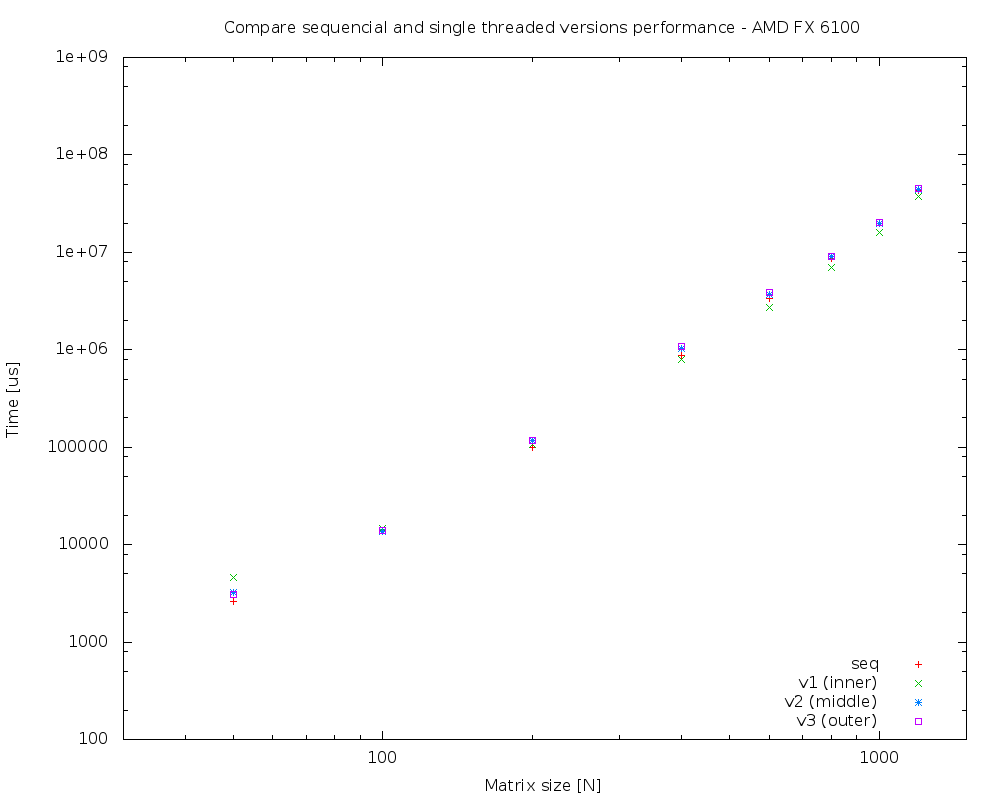
\includegraphics[width=\textwidth]{cmp_single_thread_HAL}
        \caption{HAL8k}
        \label{fig:8k_cmp_single}
    \end{subfigure}%
    ~ %add desired spacing between images, e. g. ~, \quad, \qquad, \hfill etc.
    %(or a blank line to force the subfigure onto a new line)
    \begin{subfigure}[H]{0.5\textwidth}
        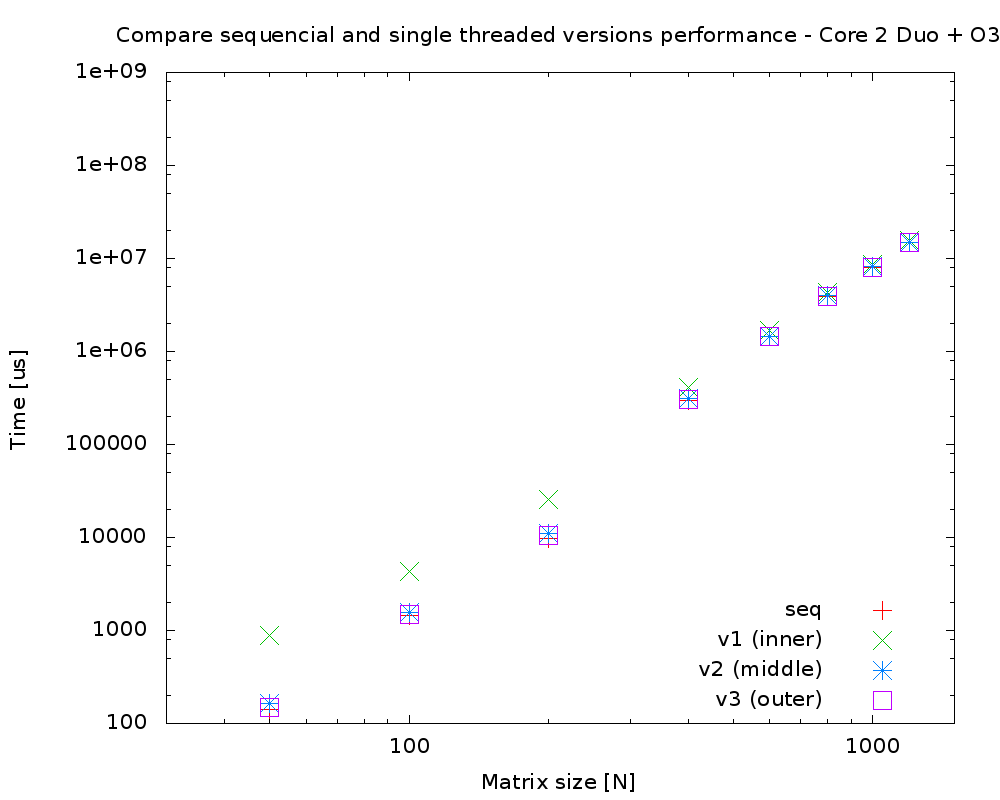
\includegraphics[width=\textwidth]{cmp_single_thread_hpops2_O3}
        \caption{hpops2\_O3}
        \label{fig:hpops2_O3_cmp_single}
    \end{subfigure}
    ~ %add desired spacing between images, e. g. ~, \quad, \qquad, \hfill etc.
    %(or a blank line to force the subfigure onto a new line)
    \begin{subfigure}[H]{0.5\textwidth}
        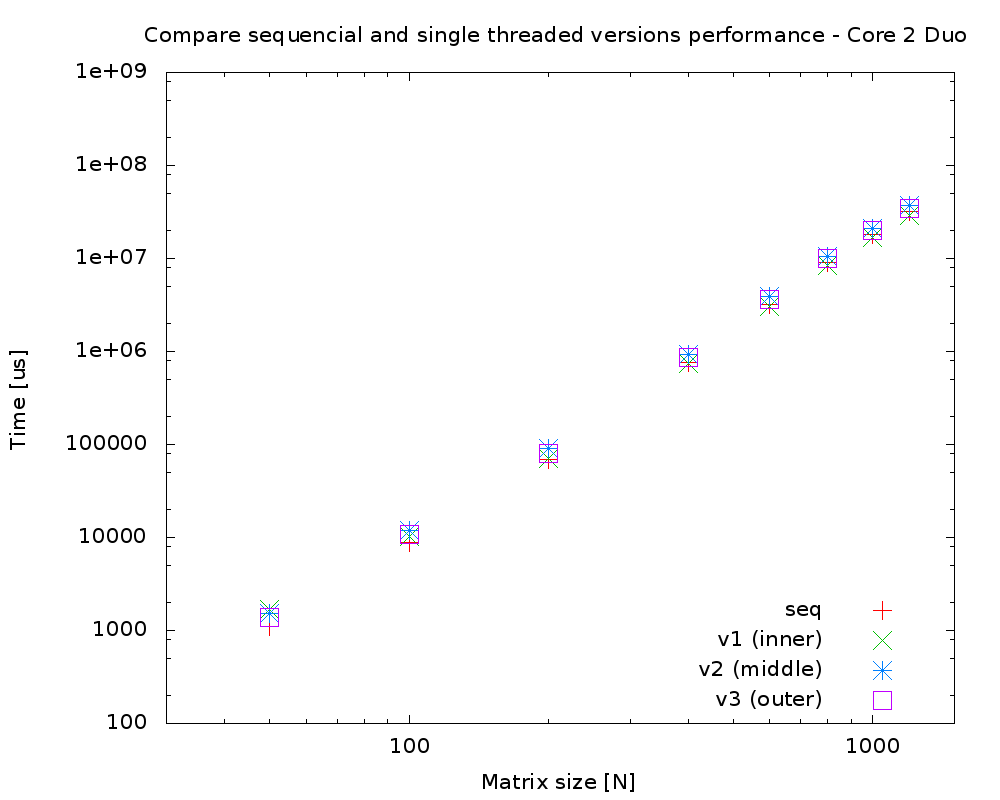
\includegraphics[width=\textwidth]{cmp_single_thread_hpops2}
        \caption{hpops2}
        \label{fig:hpops2_cmp_single}
    \end{subfigure}
    \caption{Uma \textit{thread} OpenMP vs. Algoritmo Sequencial}\label{fig:single_vs_openmp}
\end{figure}

\subsubsection{Paralelização do Laço mais Externo (de 1 a 16 \textit{threads})}

Este experimento foi realizado nas arquiteturas \textbf{hpops}
(Figuras \ref{fig:hpops2_O3_par_threads} e \ref{fig:hpops2_par_threads}),
\textbf{mops} (Figura \ref{fig:mops_par_threads}) e \textbf{HAL8k}
(Figura \ref{fig:8k_par_threads}). Utilizamos o laço mais externo
nesta comparação porque foi a modificação que apresentou os melhores
resultados em todos os experimentos.

É possível observar que a execução na arquitetura com mais \textit{cores}
(\textbf{HAL8k}, Figura \ref{fig:8k_par_threads}) se beneficiou mais
do aumento do número de \textit{threads}. Nas demais arquiteturas a
variação no número de \textit{threads} também impactou o resultado em
comparação com o programa sequencial, mas mais \textit{threads} não
implicaram num resultado muito melhor.

\begin{figure}[H]
    \centering
    \begin{subfigure}[H]{0.5\textwidth}
        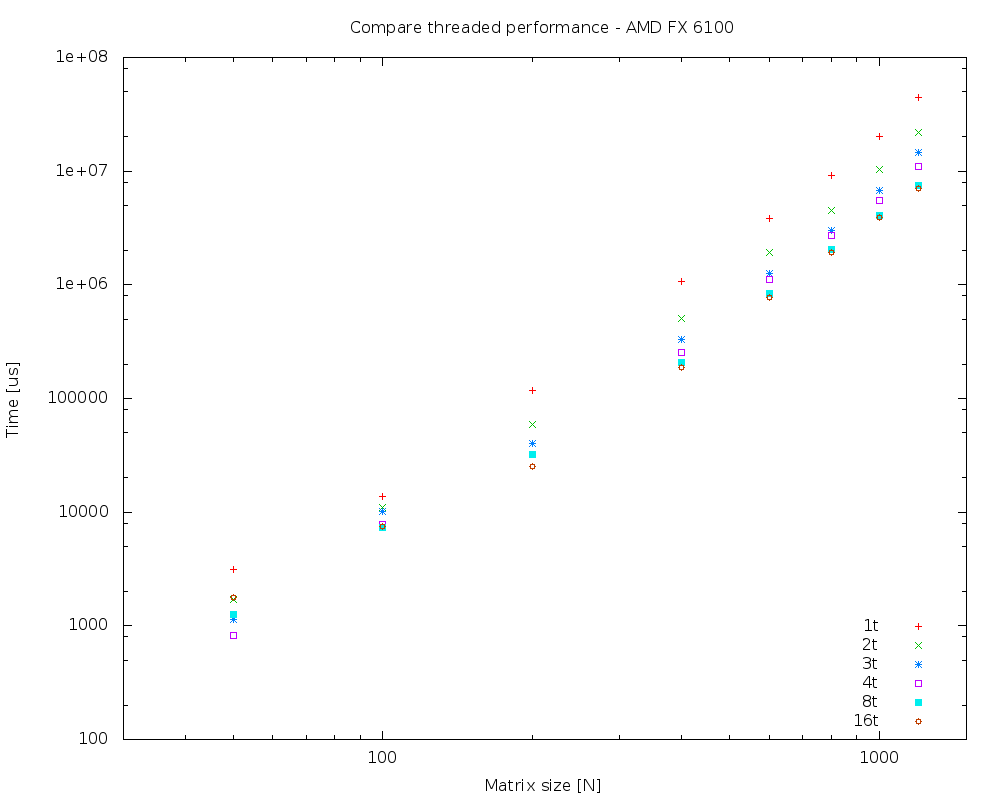
\includegraphics[width=\textwidth]{HAL_par_threads}
        \caption{HAL8k}
        \label{fig:8k_par_threads}
    \end{subfigure}%
    ~ %add desired spacing between images, e. g. ~, \quad, \qquad, \hfill etc.
    %(or a blank line to force the subfigure onto a new line)
    \begin{subfigure}[H]{0.5\textwidth}
        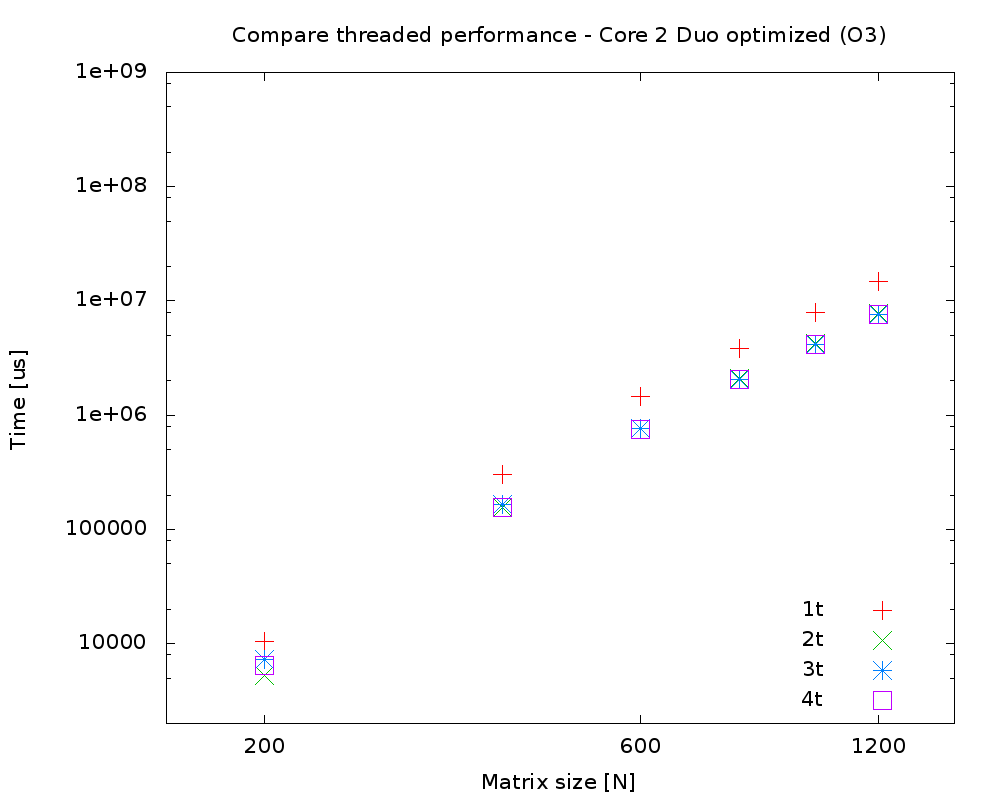
\includegraphics[width=\textwidth]{hpops2_O3_par_threads}
        \caption{hpops2\_O3}
        \label{fig:hpops2_O3_par_threads}
    \end{subfigure}
    ~ %add desired spacing between images, e. g. ~, \quad, \qquad, \hfill etc.
    %(or a blank line to force the subfigure onto a new line)
    \begin{subfigure}[H]{0.5\textwidth}
        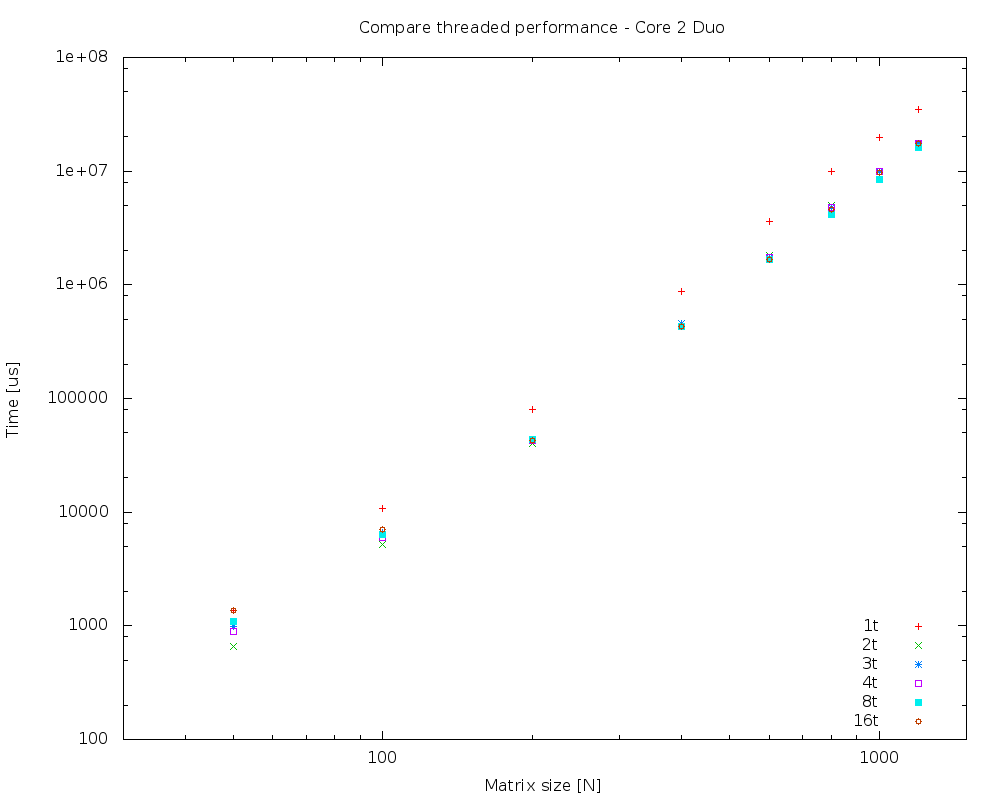
\includegraphics[width=\textwidth]{hpops2_par_threads}
        \caption{hpops2}
        \label{fig:hpops2_par_threads}
    \end{subfigure}%
    ~ %add desired spacing between images, e. g. ~, \quad, \qquad, \hfill etc.
    %(or a blank line to force the subfigure onto a new line)
    \begin{subfigure}[H]{0.5\textwidth}
        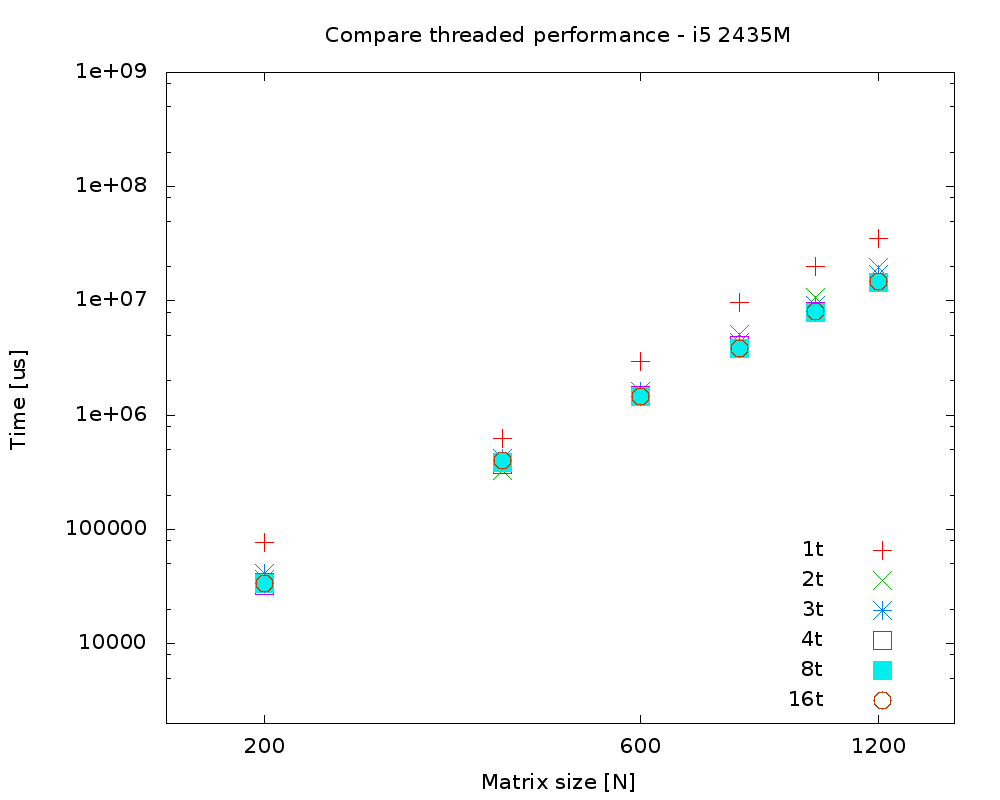
\includegraphics[width=\textwidth]{mops_par_threads}
        \caption{mops}
        \label{fig:mops_par_threads}
    \end{subfigure}
    \caption{Comparação de \textit{threads} (de 1 a 16), na paralelização do Laço mais Externo}\label{fig:animals}
\end{figure}

\subsubsection{OpenMP com 2 \textit{threads} (em todas as versões de paralelização)}

Nesta Seção apresentamos os resultados para as arquiteturas \textbf{hpops}
(Figuras \ref{fig:hpops2_O3_cmp_2t} e \ref{fig:hpops2_cmp_2t}) e \textbf{HAL8k}
(Figura \ref{fig:8k_cmp_2t}).

Neste experimento podemos observar que a paralelização do laço mais
interno, usando \textit{reduction}, teve tempo de execução menor
do que as outras versões para matrizes pequenas, mas essa diferença
diminui ao aumentar o tamanho das matrizes. Para matrizes grandes,
a paralelização do laço mais interno tem resultados mais rápidos.

\begin{figure}[H]
    \centering
    \begin{subfigure}[H]{0.5\textwidth}
        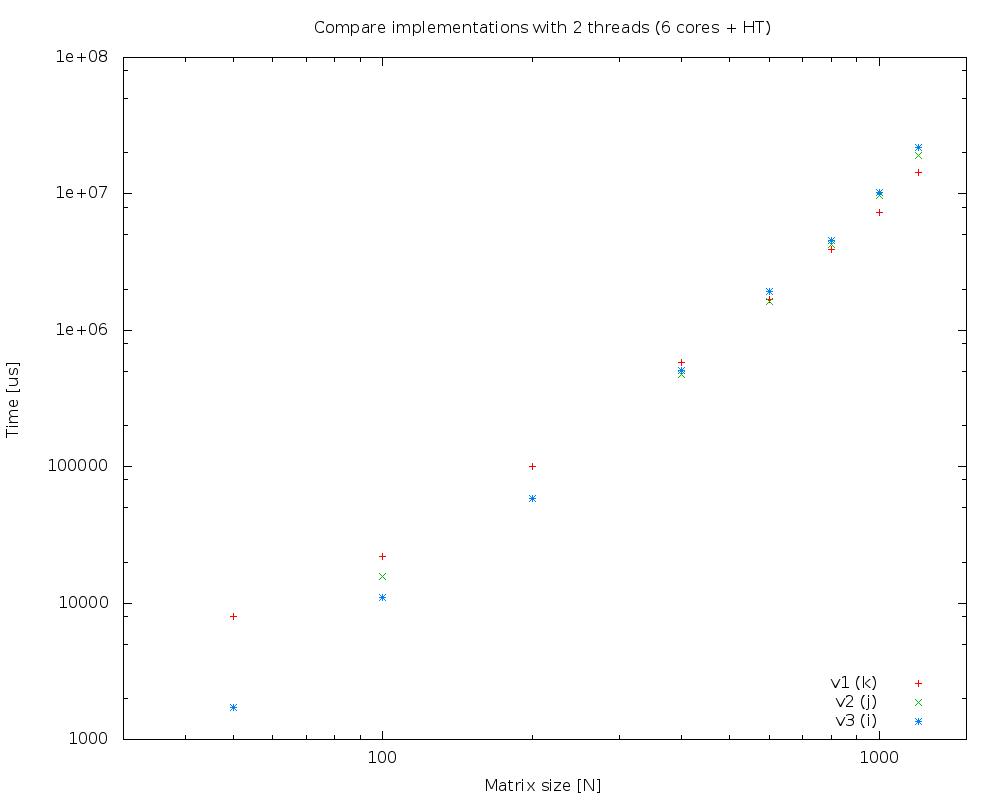
\includegraphics[width=\textwidth]{HAL_cmp_versions-2t}
        \caption{HAL8k}
        \label{fig:8k_cmp_2t}
    \end{subfigure}%
    ~ %add desired spacing between images, e. g. ~, \quad, \qquad, \hfill etc.
    %(or a blank line to force the subfigure onto a new line)
    \begin{subfigure}[H]{0.5\textwidth}
        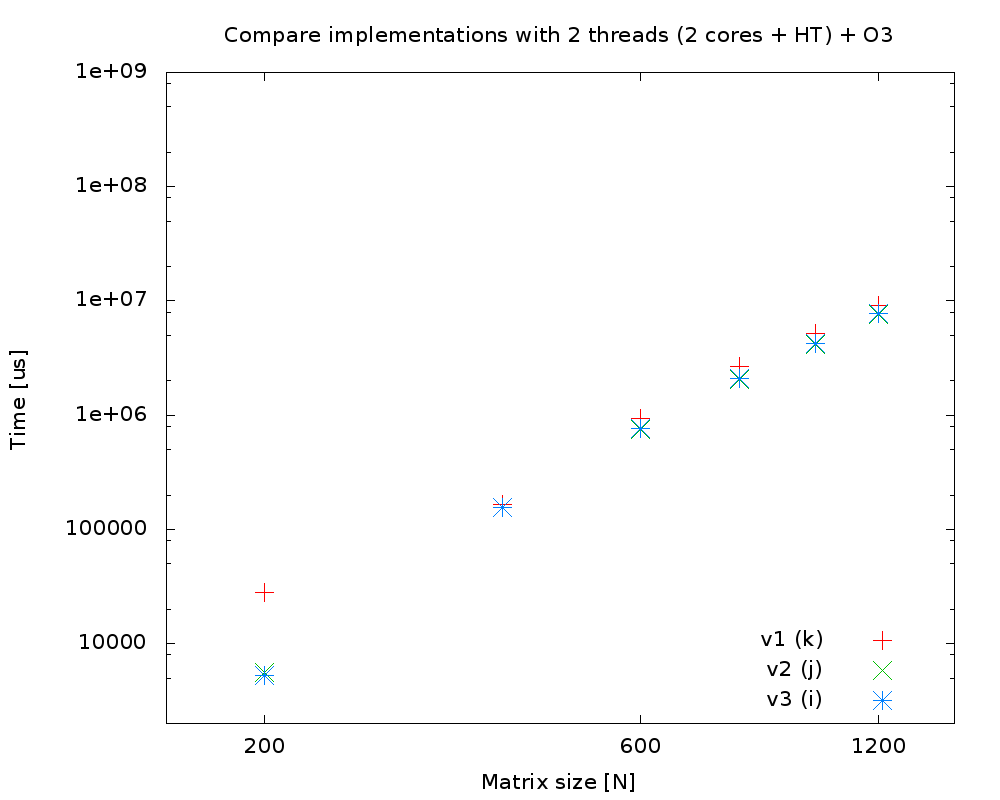
\includegraphics[width=\textwidth]{hpops2_O3_cmp_versions-2t}
        \caption{hpops2\_O3}
        \label{fig:hpops2_O3_cmp_2t}
    \end{subfigure}
    ~ %add desired spacing between images, e. g. ~, \quad, \qquad, \hfill etc.
    %(or a blank line to force the subfigure onto a new line)
    \begin{subfigure}[H]{0.5\textwidth}
        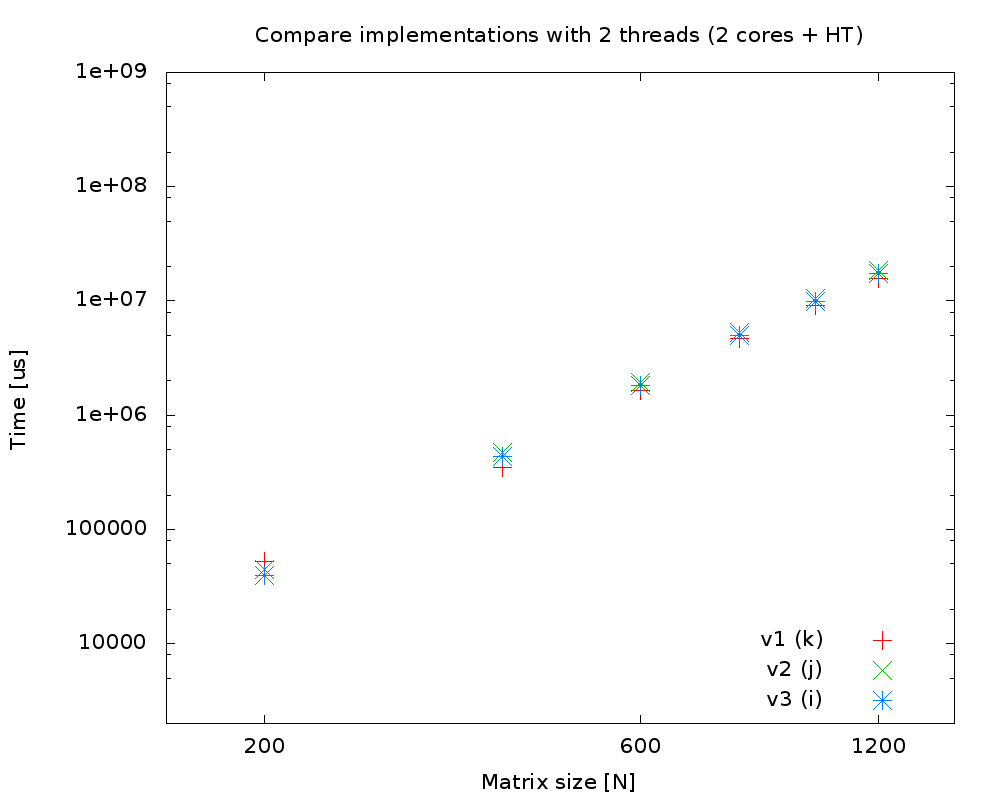
\includegraphics[width=\textwidth]{hpops2_cmp_versions-2t}
        \caption{hpops2}
        \label{fig:hpops2_cmp_2t}
    \end{subfigure}%
    \caption{OpenMP com duas \textit{threads}, em todas as versões de paralelização}\label{fig:animals}
\end{figure}

\subsubsection{OpenMP com 4 \textit{Threads} (em todas as versões de paralelização)}

Nesta Seção apresentamos os resultados para as arquiteturas \textbf{hpops}
(Figuras \ref{fig:hpops2_O3_cmp_4t} e \ref{fig:hpops2_cmp_4t}) e \textbf{HAL8k}
(Figura \ref{fig:8k_cmp_4t}).

Analogamente ao exemplo com duas \textit{threads}, vemos que a paralelização do
laço mais interno fica mais rápida conforme aumentamos o tamanho das matrizes,
em todas as arquiteturas, apesar de demorar mais para vencer as outras
paralelizações.

\begin{figure}[H]
    \centering
    \begin{subfigure}[H]{0.5\textwidth}
        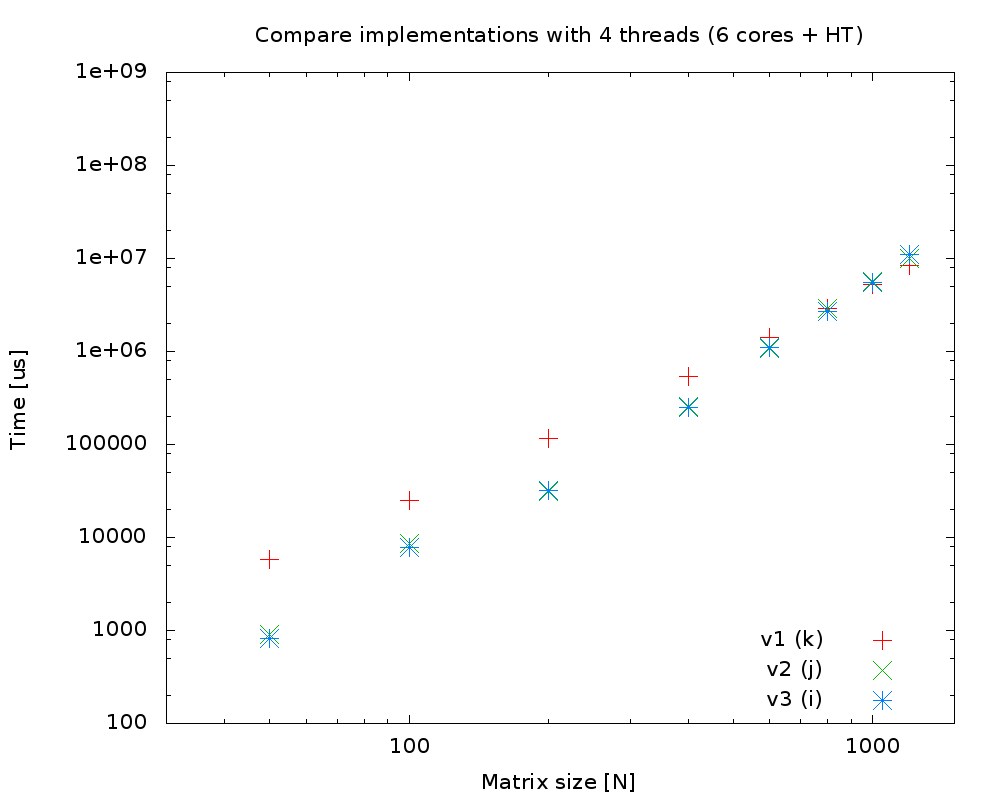
\includegraphics[width=\textwidth]{HAL_cmp_versions-4t}
        \caption{HAL8k}
        \label{fig:8k_cmp_4t}
    \end{subfigure}%
    ~ %add desired spacing between images, e. g. ~, \quad, \qquad, \hfill etc.
    %(or a blank line to force the subfigure onto a new line)
    \begin{subfigure}[H]{0.5\textwidth}
        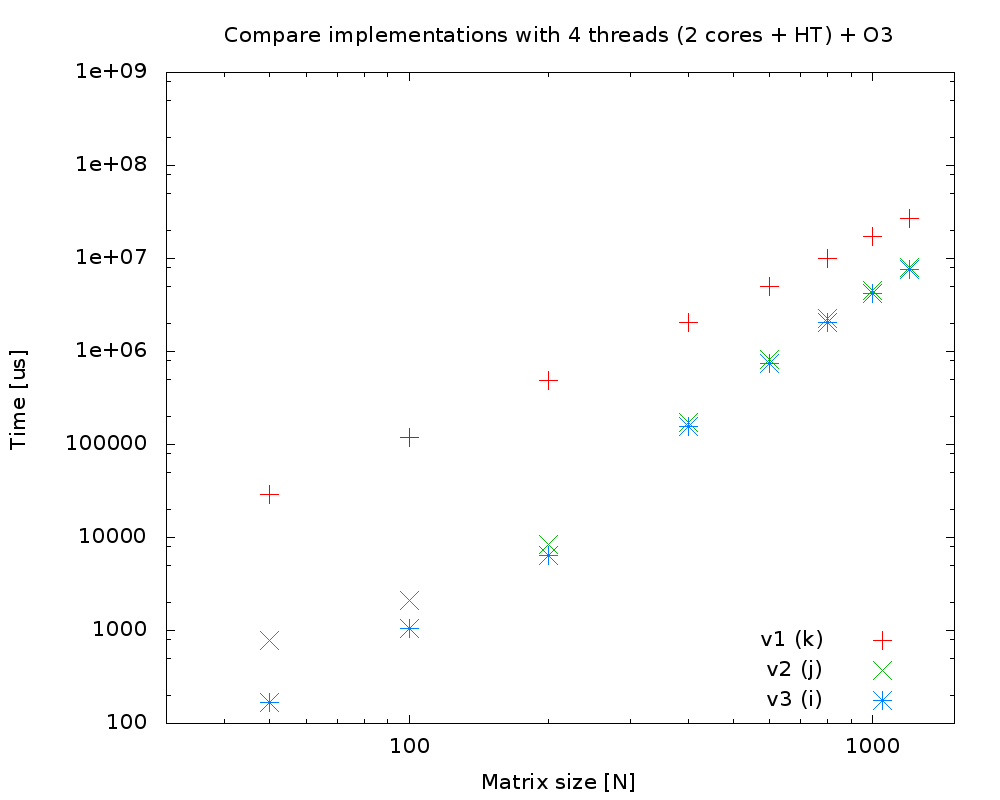
\includegraphics[width=\textwidth]{hpops2_O3_cmp_versions-4t}
        \caption{hpops2\_O3}
        \label{fig:hpops2_O3_cmp_4t}
    \end{subfigure}
    ~ %add desired spacing between images, e. g. ~, \quad, \qquad, \hfill etc.
    %(or a blank line to force the subfigure onto a new line)
    \begin{subfigure}[H]{0.5\textwidth}
        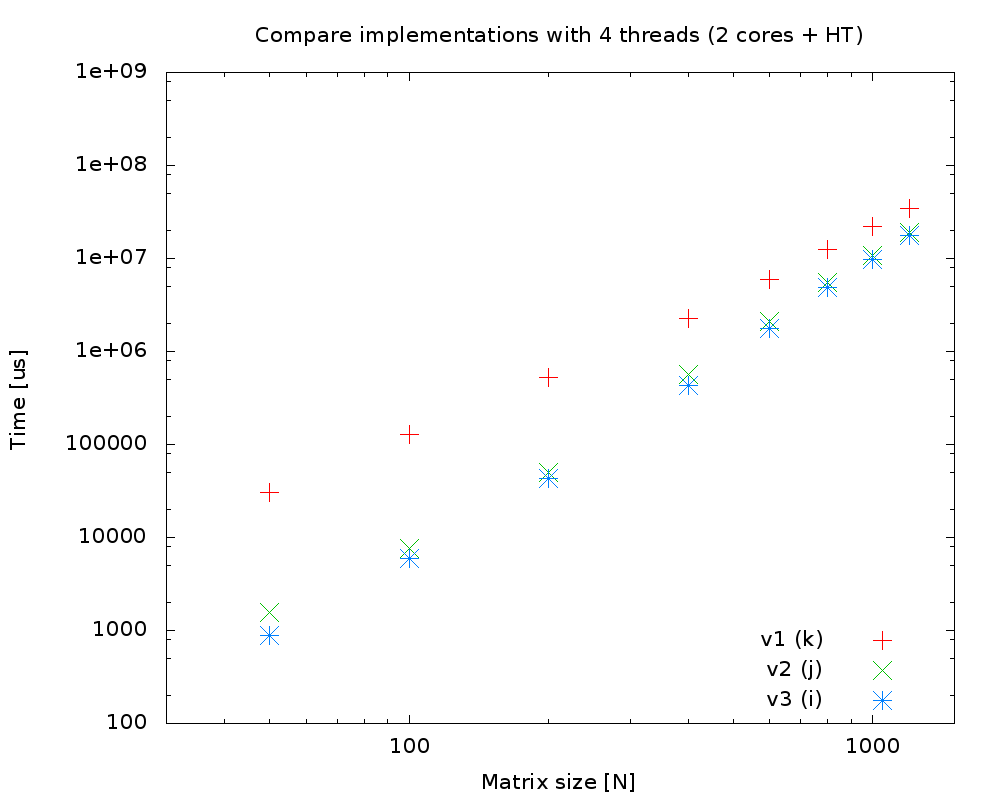
\includegraphics[width=\textwidth]{hpops2_cmp_versions-4t}
        \caption{hpops2}
        \label{fig:hpops2_cmp_4t}
    \end{subfigure}%
    \caption{OpenMP com quatro \textit{Threads}, em todas as versões de paralelização}\label{fig:animals}
\end{figure}

\subsubsection{Compilação com a \textit{flag} \texttt{-O3}}

Nesta seção vemos a comparação da execução da paralelização do laço
mais interno em relação à otimização \texttt{-O3}, na arquitetura
\textbf{hpops}. O uso da otimização sempre melhorou os resultados.

\begin{figure}[H]
    \centering
    \begin{subfigure}[H]{0.5\textwidth}
        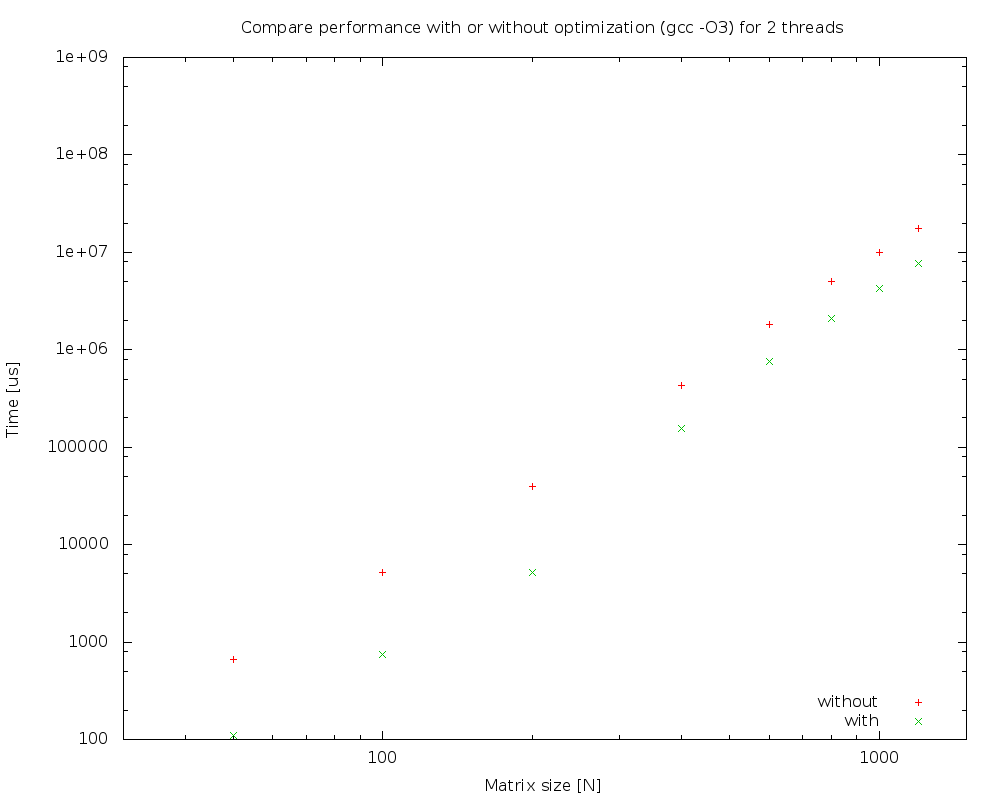
\includegraphics[width=\textwidth]{hpops_cmp_optimization-2t}
        \caption{2 \textit{threads}}
        \label{fig:hpops_o3_2t}
    \end{subfigure}%
    ~ %add desired spacing between images, e. g. ~, \quad, \qquad, \hfill etc.
    %(or a blank line to force the subfigure onto a new line)
    \begin{subfigure}[H]{0.5\textwidth}
        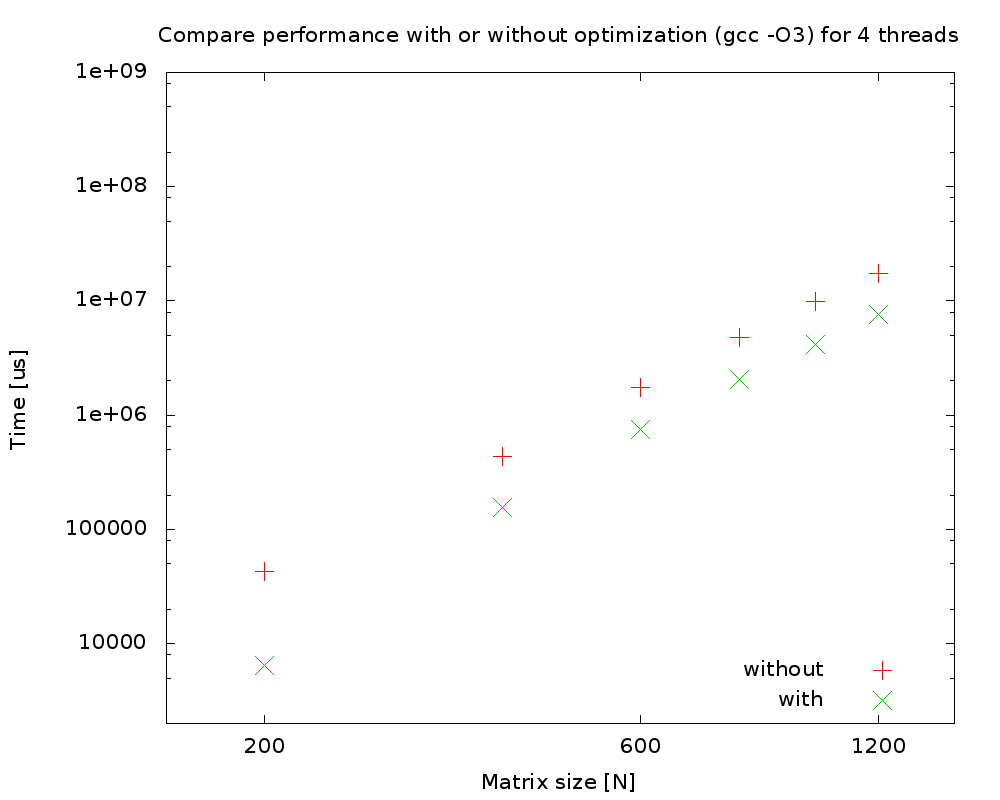
\includegraphics[width=\textwidth]{hpops_cmp_optimization-4t}
        \caption{4 \textit{threads}}
        \label{fig:hpops_o3_4t}
    \end{subfigure}
    \caption{\textbf{hpops}, compilação com a \textit{flag} \texttt{-O3}}\label{fig:animals}
\end{figure}

\subsubsection{Usando Diferentes Versões do GCC e do Kernel}

Finalmente, apresentamos resultados utilizando diferentes versões
do kernel do linux e do compilador GCC, na mesma arquitetura.
(Ver \textbf{hpops} e \textbf{hpops2}, na Seção \ref{sec:arch})

Apesar de serem versões bem próximas, é possível notar um pequeno
\textit{speedup} na versão mais nova.

\begin{figure}[H]
    \centering
    \begin{subfigure}[H]{0.5\textwidth}
        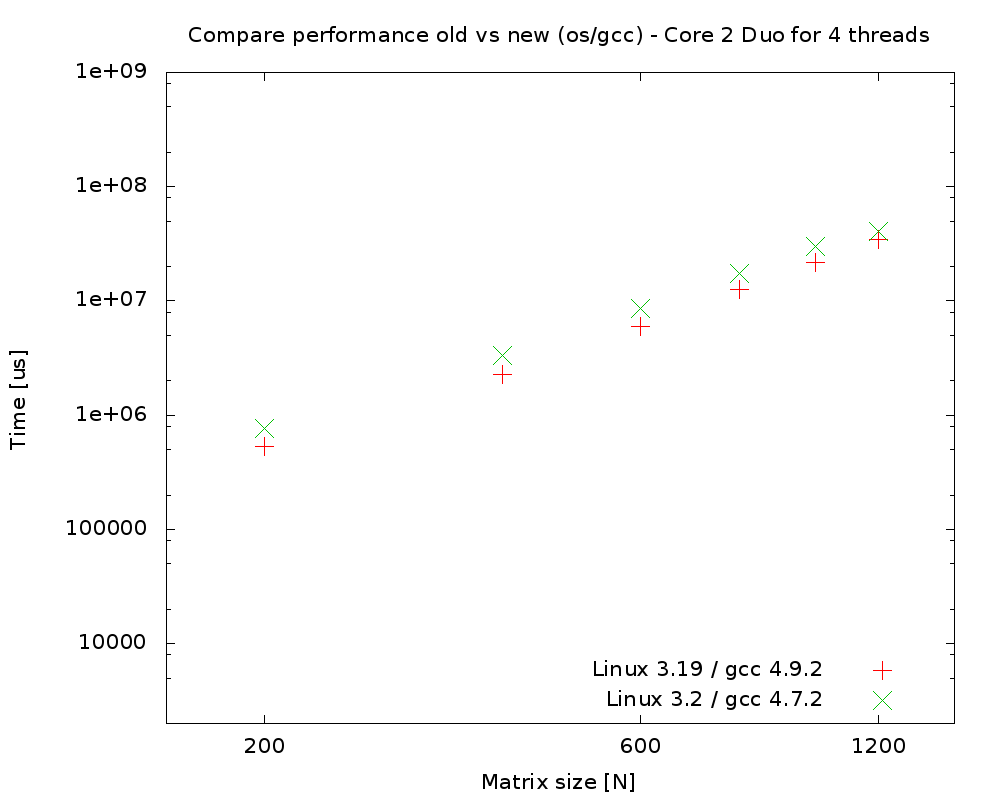
\includegraphics[width=\textwidth]{compare_old_new_os}
        \caption{hpops e hpops2}
        \label{fig:hpops_hpops2}
    \end{subfigure}%
    \caption{OpenMP em diferentes versões do GCC e Kernel}\label{fig:animals}
\end{figure}

\section{Conclusões} \label{sec:dis}



%\newpage
%\bibliographystyle{plainnat}
%\bibliography{relatorio}

\end{document}
